\begin{frame}
	\frametitle{Overleaf}
	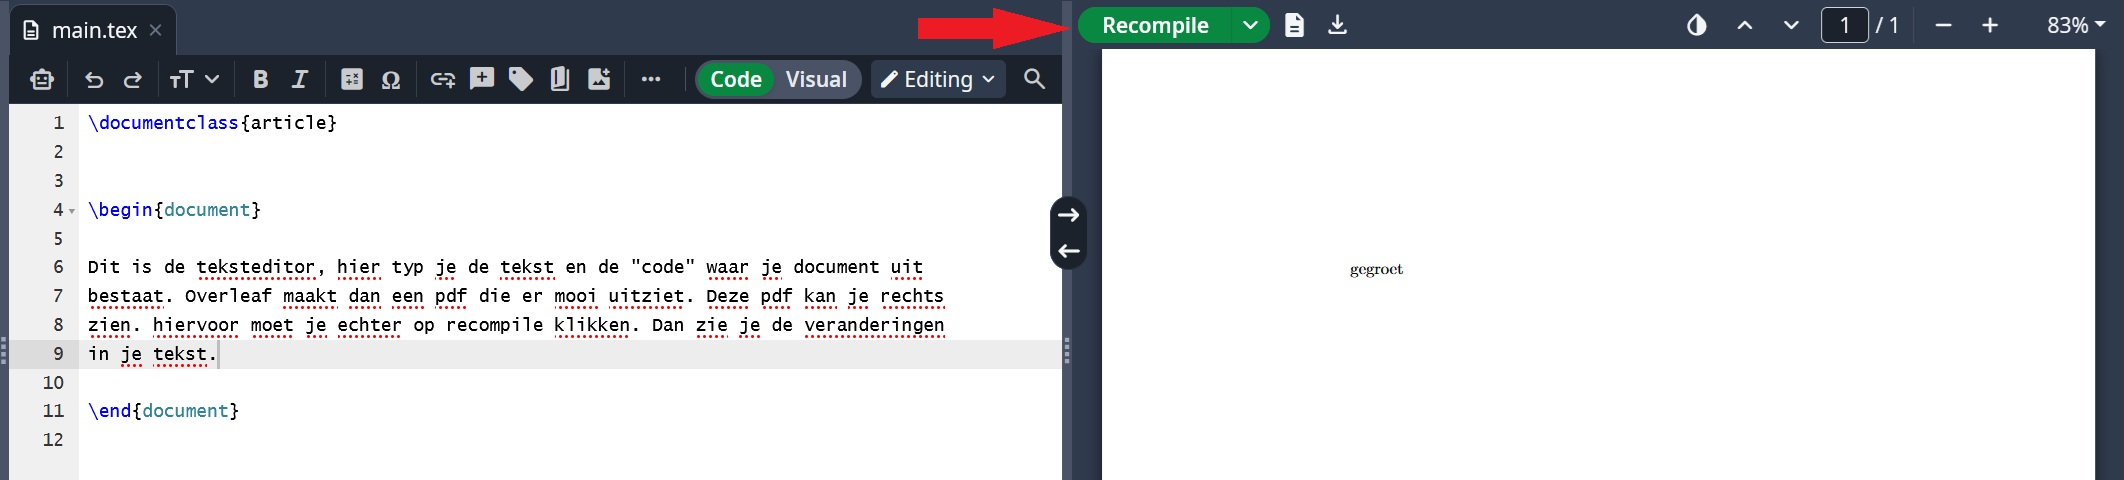
\includegraphics[width=1\textwidth]{images/recompileOverleaf.jpg}
	Links zie je de tekseditor, hier typ je de tekst en de "code" waar je document uit bestaat.
	\pause
	\newline
	Overleaf maakt dan een pdf dat er mooi uitziet. Deze pdf kan je rechts zien.
	\pause
	\newline
	Hiervoor moet je echter op recompile klikken, dan zie je de veranderingen in je tekst
\end{frame}